\documentclass[a4paper,11pt]{article}

\usepackage{mlsubmit}

\begin{document}

\initmlsubmision{2}                              					% assignment number
								{Nikhil Mittal}      						           		% your name
								{17111056}																		% your roll number

\begin{mlsolution}

1. Answer : NO. It is useful only when the Name exists in the data, but if the name is not present then we can't classify based on name. So the first attribute (name) is not useful in learning.
If we build a decision tree using the attribute name then the branching factor will be such high that it will shatter any dataset and overfit.
\\

2. Answer : Yes.\\

3. Decision Tree obtained after ID3 decision tree learning algorithm is shown in Figure 1. Steps for producing this are :
\\\\Attributes are : Size of research group, Like the research area, Average workload, No. of meetings  per week. Suppose S is this full data given. Then, \\\\Entropy(S) = 0.9182\\
Gain(S, Size of research group) = 0.0679\\
Gain(S, Like the research area) = 0.03170\\
Gain(S, Average workload) = 0.06131\\
Gain(S, No. of meetings  per week) = 0.2516\\\\So Root node is No. of meetings per week as it has the highest Gain.\\\\Since "No. of meetings per week" has three possible values, the root node has three branches (2-3, 0-1, $>$3). All rows with 2-3 meetings per week give result "NO", and similarly on taking branch "$>$3" we get "NO" as answer. \\\\We only decide on the remaining three attributes: Size of research group, Like the research area, Average workload. S is now the remaining set under branch "0-1" (No. of meetings per week).\\
Entropy(S) = 1.0\\
Gain(S, Size of research group) = 0.11452\\
Gain(S, Like the research area) = 0.0348\\
Gain(S, Average workload) = 0.439\\\\Selecting Average workload as the decision node. Splitting into branches upon its possible values. "Average" workload branch leads to always "Yes" as answer.\\Still need to decide for "Heavy" and "Light" average workload branch.\\\\For "Heavy" (Average workload) branch :\\Entropy(S) = 0.7219\\
Gain(S, Size of research group) = 0.1709\\
Gain(S, Like the research area) = 0.0729\\\\Selecting Size of research group as the decision node, highest gain.
Its branches are Medium and Large. Large always yields "NO" and Medium gives "YES" for 1 data point and "NO" for 2 data points, hence choosing "NO" by majority.\\\\For "Light" (Average workload) branch :\\
Entropy(S) = 1.0\\
Gain(S, Size of research group) = 2.0\\
Gain(S, Like the research area) = 1.0\\\\Selecting Size of research group as the decision node, highest gain. We have only Medium size as branch and it's values are "YES" and "NO" one for each data point. So arbitrarily breaking tie by choosing "YES".\\\\Since we have to stop splitting nodes that are at depth 2 or more. Hence this "Light" Average workload branch always results in "YES" as answer, hence assigning directly to "YES" without any further split. Similarly the "Heavy" Average workload branch always results in "NO" as answer irrespective of the "Size of Research group" being Medium or Large, hence directly assigning the leaf node answer "NO" without any further split.\\\\These steps give us the decision tree as shown in figure 1.

\begin{figure}[th]%
\centering
\includegraphics[width=0.5\columnwidth]{tree.png}%

\caption{Decision Tree}%
\label{fig:Dtree}%
\end{figure}



\end{mlsolution}

\begin{mlsolution}


Lorem ipsum dolor sit amet, consectetur adipiscing elit. Duis feugiat vehicula dolor, sed ultricies leo. Phasellus euismod dictum felis in euismod. Proin pretium vel neque in placerat. Proin imperdiet egestas vulputate. Etiam faucibus accumsan ante non viverra. Duis ultrices ac odio vel sodales. In maximus gravida dolor, ut commodo lacus. Pellentesque ante massa, venenatis id aliquam et, posuere sed dui. Duis dignissim justo sit amet augue posuere fringilla. Suspendisse at nisi gravida, mattis justo sit amet, elementum elit. Praesent et massa ornare, consequat dui eget, ornare risus. Duis est nibh, sollicitudin nec mattis non, mattis in leo. Donec finibus justo sed massa sagittis, non fermentum nibh dictum. Pellentesque et congue purus. Donec porta pretium porttitor.

Morbi euismod risus eu tortor ornare malesuada. Nunc sed sollicitudin neque, efficitur rhoncus tellus. Cras malesuada augue arcu. Sed sem odio, tincidunt quis laoreet ac, facilisis ut nibh. Quisque gravida dolor at egestas aliquam. Aenean mollis massa sit amet enim mattis, vel fermentum tortor facilisis. Donec pellentesque est velit, vitae posuere lorem tristique ut.

Fusce pulvinar convallis lobortis. Mauris iaculis lacus vitae dui suscipit, ut ornare neque placerat. In mattis malesuada rutrum. Vivamus consectetur tempus ex sit amet aliquam. In blandit libero at mi rutrum, nec iaculis orci cursus. Maecenas a dolor lorem. Donec pretium turpis sapien, dapibus sollicitudin odio scelerisque eget. Maecenas egestas tellus a quam scelerisque, et pretium magna condimentum. In dapibus feugiat ornare. Nunc eget nulla convallis, laoreet tortor nec, convallis dui. Etiam in leo vitae nulla facilisis congue. Curabitur blandit sodales augue. Vivamus et aliquam orci, non suscipit elit. Quisque vestibulum lacus at velit congue semper.

Nulla efficitur risus nunc, in posuere turpis tempor eget. Sed efficitur id tellus non vestibulum. Praesent elementum condimentum sollicitudin. Integer eget quam dictum, varius est sit amet, aliquam mauris. Vestibulum ante ipsum primis in faucibus orci luctus et ultrices posuere cubilia Curae; Morbi in pretium dui. Sed luctus magna rutrum ex mollis, ut blandit lacus tincidunt. In tincidunt urna neque, placerat consequat velit sagittis id. Morbi pretium maximus fermentum. Interdum et malesuada fames ac ante ipsum primis in faucibus. Duis vehicula efficitur rhoncus. Nullam lacinia semper scelerisque. Maecenas eleifend nisi et ante auctor, a tincidunt arcu molestie. Aenean faucibus feugiat arcu ac mattis.
\begin{figure}[th]%
\centering
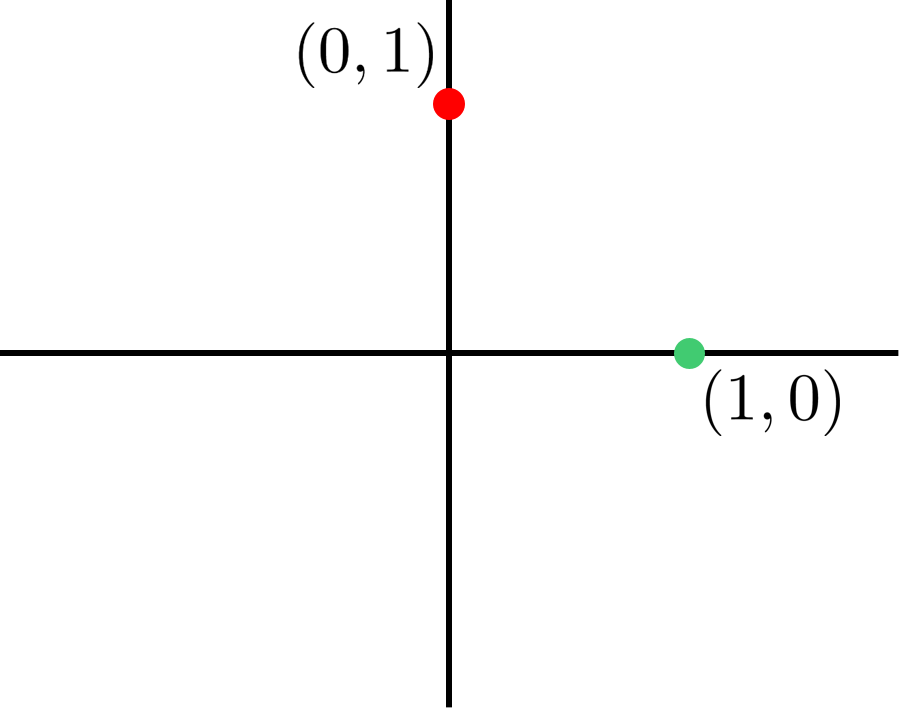
\includegraphics[width=0.5\columnwidth]{proto_blank.png}%
\hfill
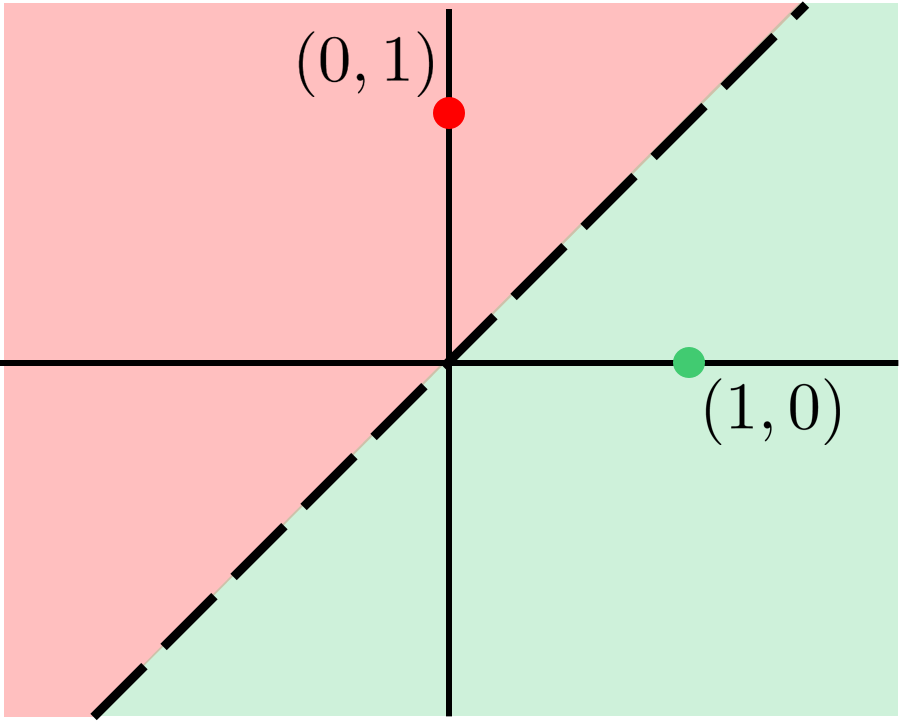
\includegraphics[width=0.5\columnwidth]{proto_euclid_sample.png}%
\caption{Learning with Prototypes: the figure on the left shows the two prototypes. The figure on the right shows what the decision boundary if the distance measure used is $d(\vz^1,\vz^2) = \norm{\vz^1-\vz^2}_2$, for any two points $\vz^1,\vz^2 \in \bR^2$. The decision boundary in this case is the line $y = x$.}%
\label{fig:proto}%
\end{figure}
Morbi quis suscipit sapien. Pellentesque pulvinar fermentum tellus at malesuada. Nam id metus vitae risus dignissim laoreet. Pellentesque massa velit, vehicula in convallis et, vestibulum sed turpis. In venenatis massa vel mattis tincidunt. Donec varius faucibus elit, in blandit metus interdum sit amet. Nullam vel nibh non nisl mollis volutpat. Donec cursus iaculis lorem, id elementum metus iaculis nec. Cras a diam porttitor, suscipit dolor id, vestibulum nisi. Morbi maximus mauris a iaculis hendrerit. Duis rutrum quam in ex lobortis gravida. Aenean iaculis lacinia metus. Fusce sit amet dignissim elit, sed sodales lacus. Mauris ac neque finibus, bibendum tortor id, scelerisque neque. In nec quam ullamcorper, egestas sem ut, iaculis ante. Nam porta diam ut lacus sagittis euismod. 
\end{mlsolution}

\begin{mlsolution}


Lorem ipsum dolor sit amet, consectetur adipiscing elit. Duis feugiat vehicula dolor, sed ultricies leo. Phasellus euismod dictum felis in euismod. Proin pretium vel neque in placerat. Proin imperdiet egestas vulputate. Etiam faucibus accumsan ante non viverra. Duis ultrices ac odio vel sodales. In maximus gravida dolor, ut commodo lacus. Pellentesque ante massa, venenatis id aliquam et, posuere sed dui. Duis dignissim justo sit amet augue posuere fringilla. Suspendisse at nisi gravida, mattis justo sit amet, elementum elit. Praesent et massa ornare, consequat dui eget, ornare risus. Duis est nibh, sollicitudin nec mattis non, mattis in leo. Donec finibus justo sed massa sagittis, non fermentum nibh dictum. Pellentesque et congue purus. Donec porta pretium porttitor.

Morbi euismod risus eu tortor ornare malesuada. Nunc sed sollicitudin neque, efficitur rhoncus tellus. Cras malesuada augue arcu. Sed sem odio, tincidunt quis laoreet ac, facilisis ut nibh. Quisque gravida dolor at egestas aliquam. Aenean mollis massa sit amet enim mattis, vel fermentum tortor facilisis. Donec pellentesque est velit, vitae posuere lorem tristique ut.

\begin{figure}[th]%
\centering
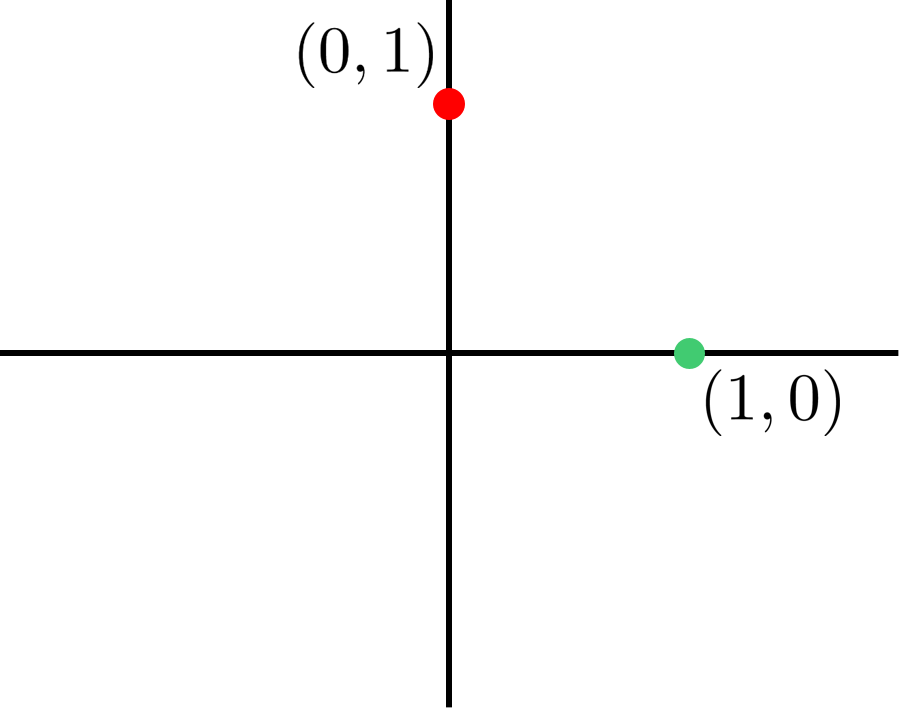
\includegraphics[width=0.4\columnwidth]{proto_blank.png}%
\hfill
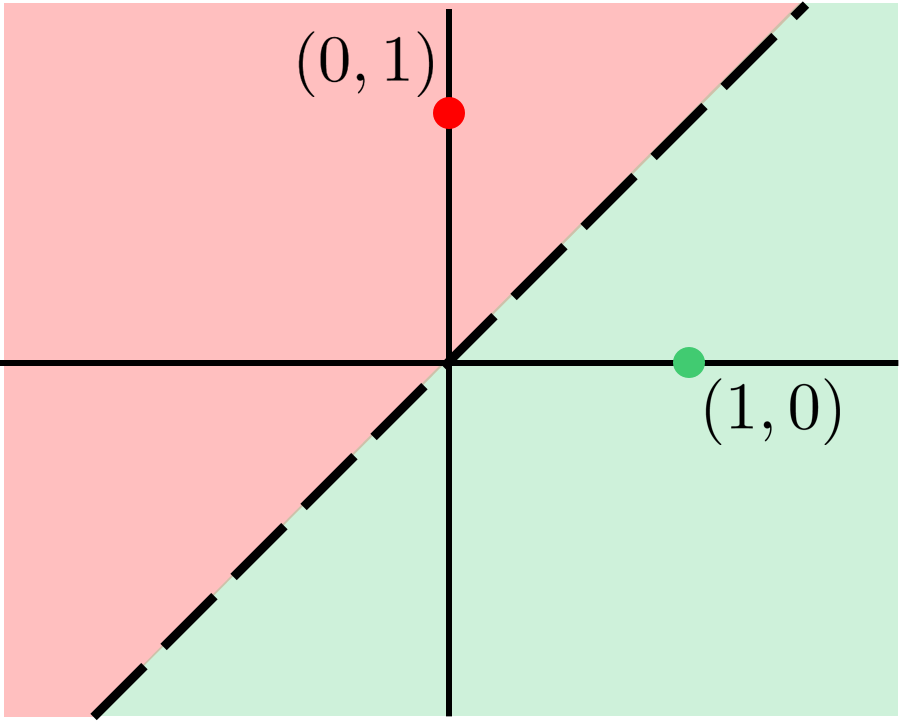
\includegraphics[width=0.4\columnwidth]{proto_euclid_sample.png}%
\caption{Learning with Prototypes: the figure on the left shows the two prototypes. The figure on the right shows what the decision boundary if the distance measure used is $d(\vz^1,\vz^2) = \norm{\vz^1-\vz^2}_2$, for any two points $\vz^1,\vz^2 \in \bR^2$. The decision boundary in this case is the line $y = x$.}%
\label{fig:proto}%
\end{figure}

Fusce pulvinar convallis lobortis. Mauris iaculis lacus vitae dui suscipit, ut ornare neque placerat. In mattis malesuada rutrum. Vivamus consectetur tempus ex sit amet aliquam. In blandit libero at mi rutrum, nec iaculis orci cursus. Maecenas a dolor lorem. Donec pretium turpis sapien, dapibus sollicitudin odio scelerisque eget. Maecenas egestas tellus a quam scelerisque, et pretium magna condimentum. In dapibus feugiat ornare. Nunc eget nulla convallis, laoreet tortor nec, convallis dui. Etiam in leo vitae nulla facilisis congue. Curabitur blandit sodales augue. Vivamus et aliquam orci, non suscipit elit. Quisque vestibulum lacus at velit congue semper.

Nulla efficitur risus nunc, in posuere turpis tempor eget. Sed efficitur id tellus non vestibulum. Praesent elementum condimentum sollicitudin. Integer eget quam dictum, varius est sit amet, aliquam mauris. Vestibulum ante ipsum primis in faucibus orci luctus et ultrices posuere cubilia Curae; Morbi in pretium dui. Sed luctus magna rutrum ex mollis, ut blandit lacus tincidunt. In tincidunt urna neque, placerat consequat velit sagittis id. Morbi pretium maximus fermentum. Interdum et malesuada fames ac ante ipsum primis in faucibus. Duis vehicula efficitur rhoncus. Nullam lacinia semper scelerisque. Maecenas eleifend nisi et ante auctor, a tincidunt arcu molestie. Aenean faucibus feugiat arcu ac mattis.

Morbi quis suscipit sapien. Pellentesque pulvinar fermentum tellus at malesuada. Nam id metus vitae risus dignissim laoreet. Pellentesque massa velit, vehicula in convallis et, vestibulum sed turpis. In venenatis massa vel mattis tincidunt. Donec varius faucibus elit, in blandit metus interdum sit amet. Nullam vel nibh non nisl mollis volutpat. Donec cursus iaculis lorem, id elementum metus iaculis nec. Cras a diam porttitor, suscipit dolor id, vestibulum nisi. Morbi maximus mauris a iaculis hendrerit. Duis rutrum quam in ex lobortis gravida. Aenean iaculis lacinia metus. Fusce sit amet dignissim elit, sed sodales lacus. Mauris ac neque finibus, bibendum tortor id, scelerisque neque. In nec quam ullamcorper, egestas sem ut, iaculis ante. Nam porta diam ut lacus sagittis euismod. 
\end{mlsolution}

\begin{mlsolution}
 Lorem ipsum dolor sit amet, consectetur adipiscing elit. Duis feugiat vehicula dolor, sed ultricies leo. Phasellus euismod dictum felis in euismod. Proin pretium vel neque in placerat. Proin imperdiet egestas vulputate. Etiam faucibus accumsan ante non viverra. Duis ultrices ac odio vel sodales. In maximus gravida dolor, ut commodo lacus. Pellentesque ante massa, venenatis id aliquam et, posuere sed dui. Duis dignissim justo sit amet augue posuere fringilla. Suspendisse at nisi gravida, mattis justo sit amet, elementum elit. Praesent et massa ornare, consequat dui eget, ornare risus. Duis est nibh, sollicitudin nec mattis non, mattis in leo. Donec finibus justo sed massa sagittis, non fermentum nibh dictum. Pellentesque et congue purus. Donec porta pretium porttitor.

Morbi euismod risus eu tortor ornare malesuada. Nunc sed sollicitudin neque, efficitur rhoncus tellus. Cras malesuada augue arcu. Sed sem odio, tincidunt quis laoreet ac, facilisis ut nibh. Quisque gravida dolor at egestas aliquam. Aenean mollis massa sit amet enim mattis, vel fermentum tortor facilisis. Donec pellentesque est velit, vitae posuere lorem tristique ut. 
\end{mlsolution}
					
\end{document}